%% =======================================================================================
%% 
%% PLANO DE PESQUISA INDIVIDUAL
%% Criado a partir da classe abntex2, desenvolvida pelo 
%% Centro de Pesquisa em Arquitetura da Informação (CPAI)
%% 
%% Arquivos de dados:   sty/configs.sty         % Configuração dos pacotes LaTeX
%%                      sty/dados_inova.sty     % Informações institucionais INOVA
%%                      sty/timbrado.sty        % Formatação do documento (layout)
%%                      sty/vocabulario.sty     % Comandos LaTeX para facilitar digitação
%%
%%                      sty/dados_pesquisa.sty  % METADADOS DO PLANO DE PESQUISA - PREENCHER!
%% 
%% =======================================================================================

\documentclass[11pt,oneside,a4paper,english,french,spanish,brazil]{abntex2}


% ----------------------------------------------------------------------------------------
% - PACOTES
  \usepackage{sty/configs}                  % Pacotes utilizados
  \usepackage{sty/dados_pesquisa}           % Definições de layout do documento
  \usepackage{sty/inova_dados}              % Dados do INOVA
  \usepackage{sty/vocabulario}              % Vocabulário específico do projeto
  \usepackage{sty/leiaute_rt}               % Definições de layout do documento
  
% ----------------------------------------------------------------------------------------

% ----------------------------------------------------------------------------------------
% - INÍCIO DO DOCUMENTO
  \begin{document}
%      \begin{sloppypar}
          
          % Seleciona o idioma do documento (conforme pacotes do babel)
            \selectlanguage{english}
            % \selectlanguage{brazil}
            
          % Retira espaço extra obsoleto entre as frases.
            \frenchspacing
          
          % ------------------------------------------------------------------------------
          % - ESTRUTURA DO DOCUMENTO
          % ------------------------------------------------------------------------------
          % ------------------------------------------------------------------------------
          % - PRÉ-TEXTUAL
          % ------------------------------------------------------------------------------
          \pagestyle{inovapre}

          % Capa
            %~~~~~~~~~~~~~~~~~~~~~~~~~~~~~~~~~~~~~~~~~~~~~~~~~~~~~~~~~~~~~~~~~~~~~
% File  : capa
%~~~~~~~~~~~~~~~~~~~~~~~~~~~~~~~~~~~~~~~~~~~~~~~~~~~~~~~~~~~~~~~~~~~~~

% Limpa os estilos de página
  \thispagestyle{empty}

% Desenho no fundo da página
  \ThisCenterWallPaper{1}{img/INOVA_capa_relatorio}

% Cria uma mini-página para inserir os dados da capa usando 70% da largura do texto
    \begin{minipage}{0.6\textwidth}
      \begin{flushleft}
          \sffamily
          % Parte superior da capa
          \vspace{2.6cm}          
          \LARGE \textbf{\ppitipo} \\
          \footnotesize \textcolor{black!60}{\ppiid} \\
          \Huge \textbf{\projpesq} \\
      \end{flushleft}
    \end{minipage}%

    \vspace{3cm}
    \begin{minipage}{0.6\textwidth}
          % Rodapé da capa
          \sffamily
          
          \rule{\textwidth}{0.2mm}
          Projeto de Pesquisa Individual vinculado ao projeto \projeto \\[0.5cm]
          Autor: \textbf{\pesquisador} \\
          Orientador: \textbf{\Orientador} \\[-0.2cm]
          \rule{\textwidth}{0.2mm}\\
    \end{minipage}%
    
    \vfill
    \begin{minipage}{0.6\textwidth}
       \ppilocal \\[0.2cm]
       \ppidata \\[0.2cm]
       \tiny Versão \ppiversao \\
    \end{minipage}%

            \clearpage
          
          % Revisões
            %~~~~~~~~~~~~~~~~~~~~~~~~~~~~~~~~~~~~~~~~~~~~~~~~~~~~~~~~~~~~~~~~~~~~~
% File  : revisoes
%~~~~~~~~~~~~~~~~~~~~~~~~~~~~~~~~~~~~~~~~~~~~~~~~~~~~~~~~~~~~~~~~~~~~~

% Tabela de revisões do plano de trabalho

    %\ABNTEXchapterfont
    \setlength{\parindent}{0cm}

    \vspace*{\fill}

    {\sffamily \Large Identificação}

        \begin{tabular}{r p{12cm}}
            \hline
            \emph{Projeto:}     & \projeto \\
            \emph{Linha de Pesquisa:} & \linhapesq \\
            \emph{Subprojeto:}  & \subprojeto \\
            \emph{Título:}      & \projpesq \\
            \emph{Id:}          & {\footnotesize  \textcolor{black!60}{\ppiid}} \\
            \emph{Pesquisador:} & \pesquisador \\
            \emph{Orientador:}  & \Orientador \\
            \emph{Data:}        & \ppidata \\
            \emph{Local:}       & \ppilocal \\
            \emph{Versão:}      & \ppiversao \\
            \hline
        \end{tabular}

    \vspace{1cm}
    {\sffamily \Large Revisões}

        \begin{scriptsize}
            \begin{tabular}{p{1.8cm}|p{8.5cm}|p{4.5cm}}
                %=============================================================
                % = CABEÇALHO
                \hline
                \textbf{Data} & \textbf{Alterações / Comentário} & \textbf{Revisor} \\ \hline
                %=============================================================

                %=============================================================
                % = REVISÕES
                2016.11.14 &
                Criação do documento. &
                Bruno Carvalho C. Souza \\ \hline

                
                %=============================================================
            \end{tabular}
        \end{scriptsize}

%----------------------------------------------------------------------

            \clearpage

          % Filiação CPAI
            %%~~~~~~~~~~~~~~~~~~~~~~~~~~~~~~~~~~~~~~~~~~~~~~~~~~~~~~~~~~~~~~~~~~~~~
% File  : filiacao_cpai
%~~~~~~~~~~~~~~~~~~~~~~~~~~~~~~~~~~~~~~~~~~~~~~~~~~~~~~~~~~~~~~~~~~~~~

%---------------------------------------------------------------------
{
\ABNTEXchapterfont\setlength{\parindent}{0cm}
\textsf{\textbf{\UnB\ -- \unb} }

{\scriptsize \textsf{\textbf{Reitora}}} \\ % {\tiny (Gestão 2012--2016)}
\textsc{\reitor}

{\scriptsize \textsf{\textbf{Vice-reitor}}}\\
\textsc{\vicereitor}


%---------------------------------------------------------------------
\vspace{0.8cm}

\textsf{\textbf{\CPAI\ -- \cpai}}

{\scriptsize \textsf{\textbf{Diretor}}}\\
\textsc{\diretorcpai}

%\vfill
%\textsf{\textbf{Pesquisador Líder}} \\
%\textsc{\ptrablider} \\
%
%\textsf{\textbf{Equipe de Pesquisa (em ordem alfabética)}}
%
%%\textsc{Ângelo Henrique Gonçalves Ramim} {\scriptsize (Analista de Tecnologia)} \\
%\textsc{Ângelo Henrique Gonçalves Ramim} \\
%\textsc{Bruno Carvalho Castro Souza} \\
%\textsc{Cláudio Roberto Vieira Chaves} \\
%\textsc{Ismael de Moura Costa} \\
%\textsc{Lauro César Araujo} \\
%\textsc{Mamede Lima-Marques} \\
%\textsc{Odilon Neves Júnior} \\
%\textsc{Paulo Argolo da Cruz Rios Filho} \\
%\textsc{Renan Lima Alves} \\
%\textsc{Romualdo Alves Pereira Junior} \\
%\textsc{Carlos Benedito Lima de Menezes} {\scriptsize (Assistente em Administração)} \\
%\textsc{Claudio Monteiro} {\scriptsize (Estagiário Técnico)} \\
%\textsc{Cláudio Roberto Vieira Chaves} {\scriptsize (Analista de Tecnologia)} \\
%\textsc{Deise de Sousa Lima} {\scriptsize (Auxiliar em Administração)} \\
%\textsc{Fabiana de Souza Damatta} {\scriptsize (Administradora)} \\
%\textsc{Jucilene Gomes Moreira} {\scriptsize (Secretária da Diretoria)} \\
%\textsc{Maria das  Dores F. Figueredo} {\scriptsize (Secretária da Diretoria)} \\
%\textsc{Moíses  Lobo de Souza Choas} {\scriptsize (Bolsista / Estagiário)} \\
%\textsc{Paulo Argolo da Cruz Rios Filho} {\scriptsize (Analista de Tecnologia)} \\
%\vspace{1cm}


%{\scriptsize \textsf{\textbf{Vice-diretor}}}\\
%\textsc{Eudes de Queiroz e Silva}

%---------------------------------------------------------------------
%\vspace{0.8cm}

%\textsf{\textbf{Centro de Seleção e de Promoção de Eventos -- CESPE}}

%{\scriptsize \textsf{\textbf{Diretor-Geral}}}\\
%\textsc{Paulo Henrique Portela}

%---------------------------------------------------------------------
%\vspace{0.8cm}

%\textsf{\textbf{Centro de  Documentação -- CEDOC}}

%{\scriptsize \textsf{\textbf{Diretora}}}\\
%\textsc{Cynthia Roncaglio}


}


%---------------------------------------------------------------------
%\clearpage

%\vspace{1cm}

%\textsf{\textbf{Grupo de Trabalho}} \hfill {\scriptsize Resolução da Reitoria n\ele\ 0068/2013}

%\vspace{1cm}

%\textsc{\mlm} -- \cpai\ -- Presidente

%\textsc{Helena Fernandes Guedes Rafael} -- \cpai\

%\textsc{Mauro Henrique de Castro} -- CESPE

%\textsc{Alexandre Schwantz} -- CESPE

%\textsc{Cynthia Roncaglio} -- CEDOC

%\cleardoublepage

%---------------------------------------------------------------------
% Fim de arquivo
%~~~~~~~~~~~~~~~~~~~~~~~~~~~~~~~~~~~~~~~~~~~~~~~~~~~~~~~~~~~~~~~~~~~~~

            %\clearpage

          % Inserir a ficha bibliografica
            %%~~~~~~~~~~~~~~~~~~~~~~~~~~~~~~~~~~~~~~~~~~~~~~~~~~~~~~~~~~~~~~~~~~~~~
%    File      : ficha_catalografica
%    Type      : TeX
%    Date      : Time-stamp: <Sunday,10 Novem 2013,18:59:18>
%
%    Content   :
%~~~~~~~~~~~~~~~~~~~~~~~~~~~~~~~~~~~~~~~~~~~~~~~~~~~~~~~~~~~~~~~~~~~~~

%----------------------------------------------------------------------
% Ficha bibliografica
%----------------------------------------------------------------------

{
\ABNTEXchapterfont\setlength{\parindent}{0cm}

\vspace*{\fill}

{\tiny \copyright\ \textit{copyright} \the\year\ CPAI -- Todos os direitos reservados}

%\imprimircassificacaoseguranca         % Não implementado nesta versão do modelo de RT

\vspace*{\fill} % Posição vertical

\begin{fichacatalografica}\ABNTEXchapterfont
    \vspace*{\fill} % Posição vertical
    \hrule % Linha horizontal
    \begin{center} % Minipage Centralizado
        \begin{minipage}[c]{13cm} % Largura
            \hspace{0.5cm} \ptrabtitulo\ / \ptrabautor. --
            \imprimirlocal : Universidade de Brasília, \ptrabdata-

            \hspace{0.5cm} \pageref{LastPage} p. : il. (algumas color.) ; 29,7 cm.\\

            \hspace{0.5cm}
            \parbox[t]{\textwidth}{\ptrabtipo~--~\CPAI, \ptrabdata.}

            \hspace{0.5cm}
            \parbox[t]{\textwidth}{Versão final.}\\

            \hspace{0.5cm}
            \parbox[t]{\textwidth}{ISSN: \ptrabissn}\\

            \hspace{0.5cm}
            1. \ptrabkeyworda.
            2. \ptrabkeywordb.
            3. \ptrabkeywordc.
            I. Título.

            \begin{flushright}
                 CDD \ptrabcdd
            \end{flushright}
        \end{minipage}
    \end{center}
    \hrule
\end{fichacatalografica}

\cleardoublepage
}

%----------------------------------------------------------------------


          % Sumarios
            \vspace{1cm}
            \tableofcontents
            
            \clearpage
            \vspace{1cm}
            \listoffigures 
            
            \vspace{1cm}
            \listoftables

            \clearpage
            
          % Lista de abreviaturas e siglas
%            %~~~~~~~~~~~~~~~~~~~~~~~~~~~~~~~~~~~~~~~~~~~~~~~~~~~~~~~~~~~~~~~~~~~~~
% File  : siglas
%~~~~~~~~~~~~~~~~~~~~~~~~~~~~~~~~~~~~~~~~~~~~~~~~~~~~~~~~~~~~~~~~~~~~~

\begin{siglas}
    \item[AEB]Agência Espacial Brasileira
    \item[AI] \AI
    \item[AIGov]  \AI\ de Governo (ou Governamental)
    \item[AIO]\AI\ Organizacional
    \item[ANA]Agência Nacional de Águas
    \item[ANEEL]  Agência Nacional de Energia Elétrica
    \item[CETESB] Companhia Ambiental do Estado de São Paulo
    \item[CI] \CI
    \item[CPAI]   \CPAI
    \item[CPTEC]  Centro de Previsão de Tempo e Estudos Climáticos
    \item[CRN]Centro Regional do Nordeste
    \item[DHN]Diretoria de Hidrografia e Navegação
    \item[FAP-DF] Fundação de Apoio a Pesquisa do Distrito Federal
    \item[Finatec] Fundação de Empreendimentos Científicos e Tecnológicos
    \item[IBP]Instituto Blaise Pascal
    \item[INMET]  Instituto Nacional de Meteorologia
    \item[INPE]   Instituto Nacional de Pesquisas Espaciais
    \item[PDTI]   Plano Diretor de Tecnologia da Informação
    \item[PoC]\emph{Proof of Concept} (Prova de Conceito)
    \item[RITLA]  Rede de Tecnologia e Informação Latino-Americana
    \item[Scientia] Cooperativa Brasileira de Ciência, Tecnologia e Inovação
    \item[TC] \tr 
    \item[TI] \TI
    %\item[UFO]\emph{Unified Fundational Onthology} (Abordagem Fundacional Unificada de Definição Ontológica)
    \item[UnB]\UnB
    \item[Unicamp] Universidade Estadual de Campinas
    
\end{siglas}
%----------------------------------------------------------------------


%%----------------------------------------------------------------------
%% Inserir Lista de símbolos
%%----------------------------------------------------------------------

\begin{simbolos}
  \item[$ \Gamma $] Letra grega Gama
  \item[$ \Lambda $] Lambda
  \item[$ \zeta $] Letra grega minúscula zeta
  \item[$ \in $] Pertence
\end{simbolos}

            
          % ------------------------------------------------------------------------------
          % - TEXTUAL
          % ------------------------------------------------------------------------------
          \pagestyle{inova}
          
          % Caracterização do projeto
            %\chapter{Caracterização do Plano de Pesquisa Individual}\label{cap:caracterizacao}
            %%~~~~~~~~~~~~~~~~~~~~~~~~~~~~~~~~~~~~~~~~~~~~~~~~~~~~~~~~~~~~~~~~~~~~~
%    File      : ppi_caracterizacao
%~~~~~~~~~~~~~~~~~~~~~~~~~~~~~~~~~~~~~~~~~~~~~~~~~~~~~~~~~~~~~~~~~~~~~


\begin{footnotesize}
    \begin{tabular}{|p{.4\textwidth}|p{.45\textwidth}|}
        \hline
        \multicolumn{2}{|p{0.85\textwidth}|}{\tiny \textbf{Projeto}} \\
        \multicolumn{2}{|p{0.85\textwidth}|}{\projeto} \\
        
        \hline
        {\tiny \textbf{Linha de Pesquisa}} & {\tiny \textbf{Subprojeto}} \\
        \linhapesq & \subprojeto \\
        
        \hline
        \multicolumn{2}{|p{0.85\textwidth}|}{\tiny \textbf{Título do Plano de Pesquisa Individual}} \\
        \multicolumn{2}{|p{0.85\textwidth}|}{\projpesq} \\
        
        \hline
        \multicolumn{2}{|p{0.85\textwidth}|}{\tiny \textbf{Pesquisador}} \\
        \multicolumn{2}{|p{0.85\textwidth}|}{\pesquisador} \\
        
        \hline
        \multicolumn{2}{|p{0.85\textwidth}|}{\tiny \textbf{Orientador}} \\
        \multicolumn{2}{|p{0.85\textwidth}|}{\Orientador} \\
        
        \hline
    \end{tabular}
\end{footnotesize}

          
          % Introdução
            \chapter{Introdução}\label{cap:introducao}
            %~~~~~~~~~~~~~~~~~~~~~~~~~~~~~~~~~~~~~~~~~~~~~~~~~~~~~~~~~~~~~~~~~~~~~
%    File      : ppi_introducao
%~~~~~~~~~~~~~~~~~~~~~~~~~~~~~~~~~~~~~~~~~~~~~~~~~~~~~~~~~~~~~~~~~~~~~

Texto de introdução do plano de pesquisa individual.

Esse texto deve apresentar os aspectos principais a serem abordados, bem como uma síntese da metodologia, se for o caso, e do contexto geral do projeto.

Também convém inserir uma breve explicação de como o plano está estruturado, suas partes e capítulos.

            
          % Problema
            \chapter{Problema}\label{cap:problema}
            %~~~~~~~~~~~~~~~~~~~~~~~~~~~~~~~~~~~~~~~~~~~~~~~~~~~~~~~~~~~~~~~~~~~~~
%    File      : ppi_problema
%~~~~~~~~~~~~~~~~~~~~~~~~~~~~~~~~~~~~~~~~~~~~~~~~~~~~~~~~~~~~~~~~~~~~~

Descreva o problema que o plano de pesquisa individual irá resolver. O problema deverá ter:

\begin{alineas}
    \item \emph{Relevância pragmática:} aplicabilidade da pesquisa individual para a instituição parceira, avaliada em função da sua aderência às necessidades institucionais e ao objeto do Plano de Trabalho do projeto; e
    
    \item \emph{Relevância científica:} importância da pesquisa individual sob a perspectiva acadêmica, avaliada em função de seu potencial de inovação científica, exploração de problemas relevantes, desenvolvimento de conceitos e proposições de modelos.    
    
    \item \emph{Relevância científica:} importância da pesquisa individual sob a perspectiva acadêmica, avaliada em função de seu potencial de inovação científica, exploração de problemas relevantes, desenvolvimento de conceitos e proposições de modelos.    
\end{alineas}


          % Justificativa
            \chapter{Justificativa}\label{cap:justificativa}
            %~~~~~~~~~~~~~~~~~~~~~~~~~~~~~~~~~~~~~~~~~~~~~~~~~~~~~~~~~~~~~~~~~~~~~
%    File      : ppi_justificativa
%~~~~~~~~~~~~~~~~~~~~~~~~~~~~~~~~~~~~~~~~~~~~~~~~~~~~~~~~~~~~~~~~~~~~~

Descreva porque esse problema é relevante cientificamente e faça um referencial teórico que embase e justifique o interesse do plano de pesquisa individual como contribuição para a solução do problema levantado.

Em outras palavras, justifique -- pragmática e cientificamente -- porque o seu plano de pesquisa vale a pena ser executado.

          % Justificativa
            \chapter{Objetivos}\label{cap:objetivos}
            %~~~~~~~~~~~~~~~~~~~~~~~~~~~~~~~~~~~~~~~~~~~~~~~~~~~~~~~~~~~~~~~~~~~~~
%    File      : ppi_objetivos
%~~~~~~~~~~~~~~~~~~~~~~~~~~~~~~~~~~~~~~~~~~~~~~~~~~~~~~~~~~~~~~~~~~~~~

\section{Objetivo Geral}\label{sec:objetivo_geral}

O objetivo geral deve estar alinhado à proposta da linha de pesquisa e do subprojeto ao qual o plano de pesquisa individual está atrelado.


\section{Objetivos Específicos}\label{sec:objetivos_especificos}

\begin{alineas}
    \item Objetivo específico 1.
    
    \item Objetivo específico 2.
    
    \item Objetivo específico 3.
    
    \item Objetivo específico 4.
\end{alineas}


          % Metodologia
            \chapter{Metodologia}\label{cap:metodologia}
            %~~~~~~~~~~~~~~~~~~~~~~~~~~~~~~~~~~~~~~~~~~~~~~~~~~~~~~~~~~~~~~~~~~~~~
%    File      : ppi_metodologia
%~~~~~~~~~~~~~~~~~~~~~~~~~~~~~~~~~~~~~~~~~~~~~~~~~~~~~~~~~~~~~~~~~~~~~

Detalhar a metodologia que será utilizada para o desenvolvimento do plano de pesquisa individual. Como referência, apresenta-se o \MAIA\ -- \maia, utilizado pelo \inova.

A metodologia utilizada para o desenvolvimento do projeto utilizará o \MAIA\ (\maia) \cite{costa_um_2010}, cujo conceito simplificado é apresentado na \autoref{fig:maia}.

\begin{figure}[H]
  \centering
  \caption[\maia]{\MAIA\ -- \maia}\label{fig:maia}
  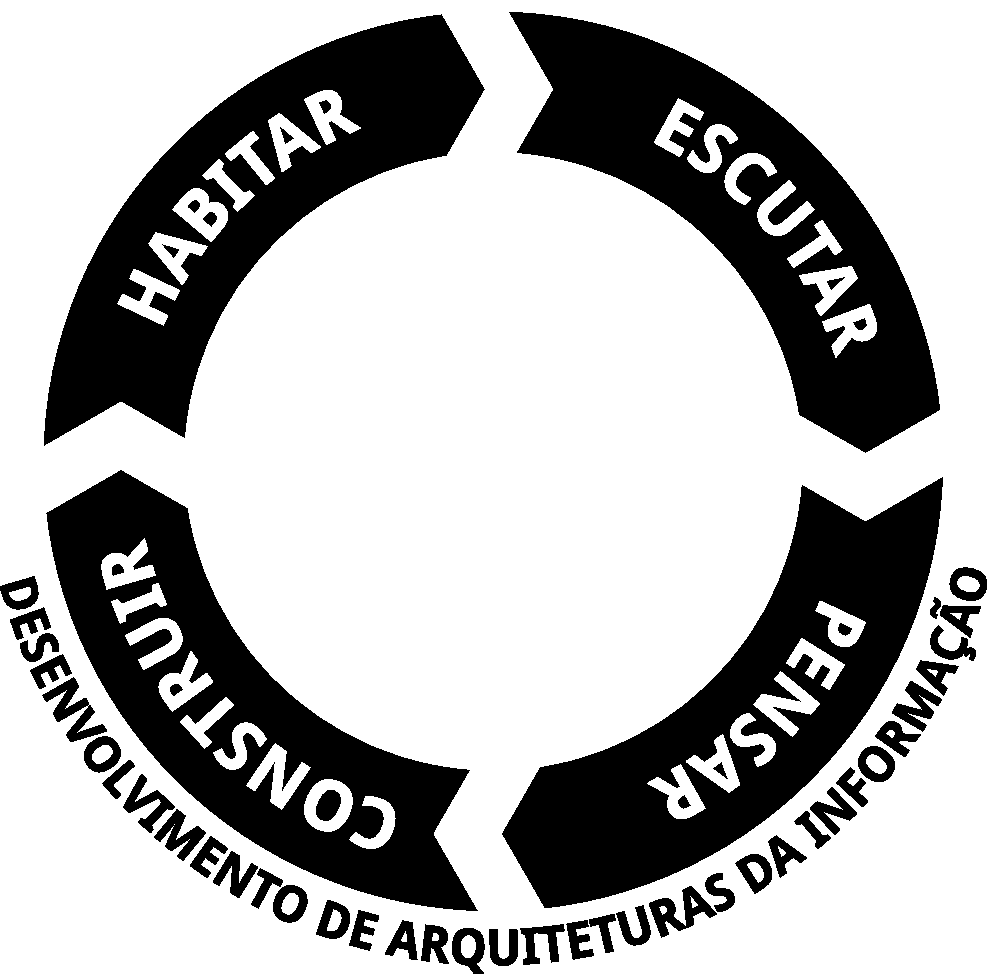
\includegraphics[width=0.4\linewidth,frame=0.5pt 5pt]{img/maia}
  \fonte{Equipe de pesquisa -- \textsc{cpai} (2016)}
\end{figure}

O Escutar, o Pensar, o Construir e o Habitar são momentos de atuação do sujeito sobre um espaço de informação. O Escutar e o Pensar são momentos voltados para os aspectos abstratos deste espaço. O Construir e o Habitar são momentos voltados para os aspectos concretos. O Escutar é o momento que concentra as percepções do espaço de informação. O Pensar concentra a modelagem hermenêutica de um espaço de informação. O Construir reúne as ações de manipulação dos elementos de um espaço de informação. O Habitar é o momento no qual o sujeito usa o espaço de informação percebido, modelado e aperfeiçoado com suas intenções. A configuração dos elementos em um espaço de informação é denominado de \AI\ (\ai).


\section{Percurso Metodológico}\label{sec:percurso_metodologico}

Etapas necessárias para o desenvolvimento do plano. Segue referência:

Esta pesquisa possuirá abordagem explicativa e qualitativa. Os procedimentos técnicos adotados serão bibliográfico, estatístico e estudo de caso. O percurso metodológico seguirá o seguinte caminho:

\begin{alineas}
    \item Levantamento bibliográfico e análise nas áreas relevantes;
    
    \item Investigação qualitativa para a análise da formação do juízo de valor em usuários de repositórios digitais e as circunstâncias de uso desses repositórios;
    
    \item Estabelecimento de relações entre as abordagens teóricas e a investigação qualitativa, buscando encontrar pontos de convergência e distanciamento entre a visão conceitual e a aplicação pragmática;

    \item Validação do modelo proposto em base empírica.
\end{alineas}



          % Aspectos de Inovação
            \chapter{Aspectos de Inovação}\label{cap:inovacao}
            %~~~~~~~~~~~~~~~~~~~~~~~~~~~~~~~~~~~~~~~~~~~~~~~~~~~~~~~~~~~~~~~~~~~~~
%    File      : ppi_aspectos_inovacao
%~~~~~~~~~~~~~~~~~~~~~~~~~~~~~~~~~~~~~~~~~~~~~~~~~~~~~~~~~~~~~~~~~~~~~

A Lei n\ele\ 13.243/2016, em seu Art. 2\ele, caracteriza inovação como ``introdução de novidade ou aperfeiçoamento no ambiente produtivo e social que resulte em novos produtos, serviços ou processos ou que compreenda a agregação de novas funcionalidades ou características a produto, serviço ou processo já existente que possa resultar em melhorias e em efetivo ganho de qualidade ou desempenho''.

Com base nessa definição, a pesquisa \projpesq\ apresenta as seguintes características e aspectos inovadores:

\begin{alineas}
    \item Característica inovadora 1.

    \item Característica inovadora 2.

    \item Característica inovadora 3.

    \item Característica inovadora 4.
\end{alineas}

            
          % Cronograma
            \chapter{Cronograma Físico}\label{cap:cronograma}
            %~~~~~~~~~~~~~~~~~~~~~~~~~~~~~~~~~~~~~~~~~~~~~~~~~~~~~~~~~~~~~~~~~~~~~
%    File      : ppi_cronograma
%~~~~~~~~~~~~~~~~~~~~~~~~~~~~~~~~~~~~~~~~~~~~~~~~~~~~~~~~~~~~~~~~~~~~~

A  \autoref{fig:cronograma} apresenta o cronograma de execução da pesquisa.

\begin{figure}[H]
    \caption{Cronograma do Projeto}\label{fig:cronograma}
    \begin{ganttchart}[
        y unit title=0.7cm,
        y unit chart=0.6cm,
        x unit=0.65cm,
        title/.append style={draw=none, fill=black!80},
        title label font=\sffamily\color{white},
        title label node/.append style={below=-1.6ex},
        title height=1,
        bar/.append style={draw=none, fill=black!50},
        bar height=.5,
        bar label font=\sffamily\footnotesize\color{black!50},
        group right shift=0,
        group top shift=.6,
        group height=.3,
        group peaks height=.2,
        group label font=\sffamily,
        milestone label font=\sffamily\footnotesize\color{black!80},
        bar incomplete/.append style={fill=maroon},
        hgrid=true,vgrid=true,
        canvas/.style=%
        {shape=rectangle, draw=black!70, dashed, thick}
        ]{1}{16}
        
        \gantttitle{Anos / Trimestres}{16} \\
        \gantttitle{1º Ano}{4} \gantttitle{2º Ano}{4} \gantttitle{3º Ano}{4} \gantttitle{4º Ano}{4} \\
        \gantttitlelist{1,...,16}{1} \\
        
        \ganttgroup{Revisão de Literatura}{1}{8} \\
        \ganttbar{Comunicação}{1}{8} \\
        \ganttbar{Arquitetura da Informação}{1}{7} \\
        \ganttbar{Ontologias}{1}{5} \\
        \ganttmilestone{Artigo 1}{4} \\
        \ganttbar{Big Data fotográfico}{5}{7} \\
        \ganttbar{Outros temas de interesse}{5}{7} \\
        \ganttmilestone{Artigo 2}{7} \\
        \ganttbar{Aspectos emocionais e cognitivos}{5}{8} \\
        \ganttbar{Métodos de pesquisas qualitativas}{5}{8} \\
        \ganttmilestone{Defesa de Qualificação}{8} \\
        
        \ganttgroup{Pesquisa Qualitativa}{9}{12} \\
        \ganttbar{Planejamento}{9}{10} \\
        \ganttbar{Aplicação}{10}{10} \\
        \ganttbar{Interpretação e relatórios}{11}{12} \\
        \ganttmilestone{Artigo 3}{12} \\
        
        \ganttgroup{Elaboração de Modelos}{13}{16} \\
        \ganttbar{Fundamentação e detalhamento}{13}{14} \\
        \ganttbar{Critérios para validação}{13}{14} \\
        \ganttbar{Aplicação}{14}{15} \\
        \ganttbar{Validação}{15}{16} \\
        \ganttmilestone{Artigo 4}{15} \\
        \ganttmilestone{Defesa de Tese}{16}
        
    \end{ganttchart}
\end{figure}


            
          % Impacto e Resultados Esperados
            \chapter{Impacto e Resultados Esperados}\label{cap:impacto}
            %~~~~~~~~~~~~~~~~~~~~~~~~~~~~~~~~~~~~~~~~~~~~~~~~~~~~~~~~~~~~~~~~~~~~~
%    File      : ppi_impacto
%~~~~~~~~~~~~~~~~~~~~~~~~~~~~~~~~~~~~~~~~~~~~~~~~~~~~~~~~~~~~~~~~~~~~~

Descreva os impactos e resultados esperados pela pesquisa.
          
          % Considerações Finais
            \chapter{Considerações Finais}\label{cap:conclusao}
            %~~~~~~~~~~~~~~~~~~~~~~~~~~~~~~~~~~~~~~~~~~~~~~~~~~~~~~~~~~~~~~~~~~~~~
%    File      : ppi_conclusao
%~~~~~~~~~~~~~~~~~~~~~~~~~~~~~~~~~~~~~~~~~~~~~~~~~~~~~~~~~~~~~~~~~~~~~

Considerações finais sobre o plano de pesquisa. Aqui você deve incluir suas observações sobre os resultados esperados, discutir as implicações da pesquisa, relacionar a pesquisa com outras iniciativas da mesma linha de pesquisa / subprojeto e fazer outros apontamentos. Também é possível incluir aspectos sobre estudos e trabalhos futuros.


          % ------------------------------------------------------------------------------
          % - PÓS-TEXTUAL
          % ------------------------------------------------------------------------------
          \pagestyle{inovapre}
        
          % Referências bibliográficas
            \clearpage
            \bibliography{bib/ppi}
        
          % Glossário
            %\glossary              % Consulte o manual da classe abntex2 para orientações sobre o glossário.

          % Apêndices
            %\part*{Apêndices}
            %\begin{apendicesenv}

                %\chapter{Título do Apêndice}\label{apend:apendice1}
                %\input{pos-textual/apend01}

            %\end{apendicesenv}
                
          % Anexos
            % \part*{Anexos}
            % \begin{anexosenv}

                

            % \end{anexosenv}
          
          % Índice remissimo
            \printindex

%    \end{sloppypar}
\end{document}
